\section{Experimentation}
\label{sec:experiments}

In this section we examine the properties of \SCAMPLON{} and compare them to
properties of \CYCLON{}, a state-of-the-art cyclic peer sampling service.  As
\CYCLON{} uses fixed-sized partial views, we must predefine its partial view
size $c$.  As shown by Erd{\H o}s and R{\' e}nyi\cite{erdos1959random} random
graphs with less than $(|\mathcal{N}|*\ln|\mathcal{N}|)$ connections are likely
to partition - which is not desired for random peer sampling services.  We want
\CYCLON{} to be optimal for a network size of 1000 peers so we set the partial
view size to $c=7\approx \ln{1000}$ while in each cycle we exchange $l=3$
peers.  We call \CYCLON{} undersized when $\ln{|\mathcal{N}}| > c$, oversized
when $\ln{|\mathcal{N}|} < c$ and optimal when $\ln{|\mathcal{N}|} \approx c$.
The experiments\footnote{Implementation:
  https://github.com/anonymous/anonymous4now} involve up to 500,000 nodes and
are carried out on \PEERSIM{} \cite{peersim}, a simulator for peer-to-peer
networks.  We define a cycle as $\Delta t$ in which each peer has executed its
active protocol once.

We inspect three properties characteristic for random graphs, the \emph{average
  clustering coefficient}~\ref{subsec:cluster}, the \emph{average shortest path
  length}~\ref{subsec:avg} and \emph{the partial view size
  distribution}~\ref{subsec:dist}. Additionally, we investigate on
\emph{robustness to random failures}.

\subsection{Clustering coefficient}
\label{subsec:cluster}

\begin{figure}
  \centering
  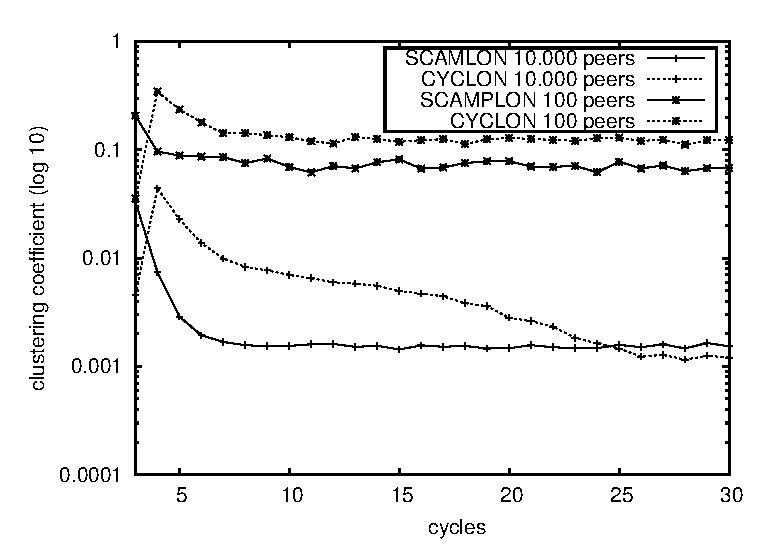
\includegraphics[width=0.49\textwidth]{img/cluster.eps}
  \caption{\label{fig:clustering}Clustering coefficient}
\end{figure}

\begin{asparadesc}
\item[Objective:] We want to evaluate to what degree \SCAMPLON{} generates
  clusters in the overlay.  To satisfy the random peer sampling objective it is
  desired that the network has few clusters, thus has a sufficiently low
  clustering coefficient.  This is important for various reasons: first: highly
  clustered networks show poor load-balancing when messages are broadcast as
  peers have a high chance of receiving a message multiple times through their
  neighbors; and second: A network consisting of poorly connected clusters is
  less robust regarding peers failing or simply leaving the overlay to
  disconnect the graph.
\item[Description:] The average clustering coefficient $\overline{C}$ measures
  the connectivity of each peer's neighborhood in the network.
  \begin{equation}
    \overline{C} = {1\over |\mathcal{N}|}\sum\limits_{x\in\mathcal{N}}C_x
  \end{equation}
  where $C_x$ is the local clustering coefficient of Peer $p_x$. The higher the
  coefficient, the more likely the network contains cliques.  The experiments
  involve 100, 1000, 10000 and 100000 peers.
\item[Results:] Figure \ref{fig:clustering} shows that \SCAMPLON{} converges
  faster than \CYCLON{}.  Furthermore, oversized \CYCLON{} converges to a
  higher value than \SCAMPLON while it converges to a lower one when
  undersized.
\item[Reasons:] The experiments yield the expected results: \SCAMPLON{}
  converges faster as it is not constraint by a fixed, artificial barrier
  $l$.  On the other hand, \CYCLON{} yields a lower clustering coefficient on
  convergence when undersized.  This can be explained by the fact that peers in
  an undersized \CYCLON{} overlay have less connections and thus have a lower
  probability of forming cliques.  This, however, makes it more vulnerable to
  node failure and churn.
\end{asparadesc}

\subsection{Average path length}
\label{subsec:avg}
\begin{figure}
  \centering
  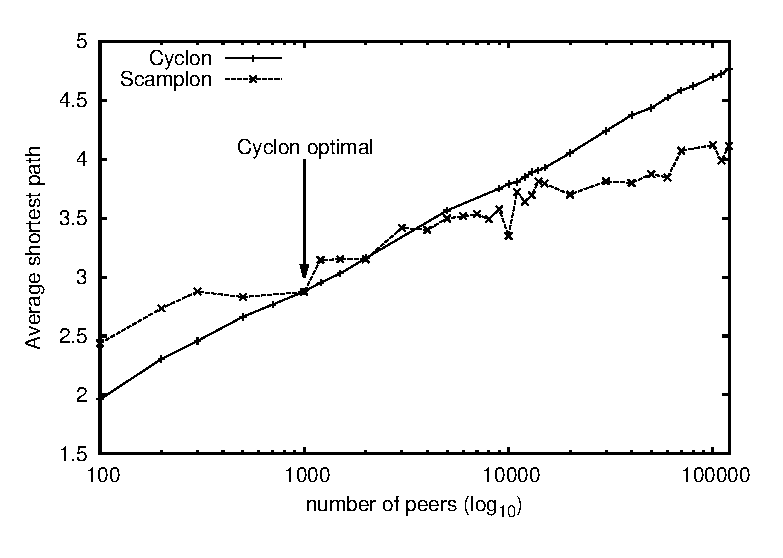
\includegraphics[width=0.49\textwidth]{img/avgpath.eps}
  \caption{\label{fig:avgpath}Average shortest path}
\end{figure}

\begin{asparadesc}
\item[Objective:] In this experiment we examine the shortest path length that
  peers have to all other nodes in the network.  Messages should disseminate
  quickly into the network which makes it crucial that the shortest path to
  other peers is, in fact, short.
\item[Description:] The average path length is the average of the shortest path
  length between peers in the graph. It counts the minimum number of hops to
  reach a peer from another given peer.  For performance reasons, we select a
  subset of 7 nodes, calculate their average shortest path and average it by 7.
\item[Results:] Figure~\ref{fig:avgpath} shows that \CYCLON{}, when oversized,
  yield a shorter average path length then \SCAMPLON{} but is quickly exceeded
  when undersized.
  %after its optimal partial view size is exceeded \SCAMPLON{} yields a shorter
  %path.
\item[Reasons:] While oversized \CYCLON{} is much better connected into the
  graph and thus yields a lower average path length then \SCAMPLON{}, as soon
  as it is undersized, \SCAMPLON{} is, thanks to bigger partial views, better
  connected into the graph and, consequently, yields the shorter average path
  length.
\end{asparadesc}

\subsection{Partial view size distribution}
\label{subsec:dist}

\begin{figure}
  \centering
  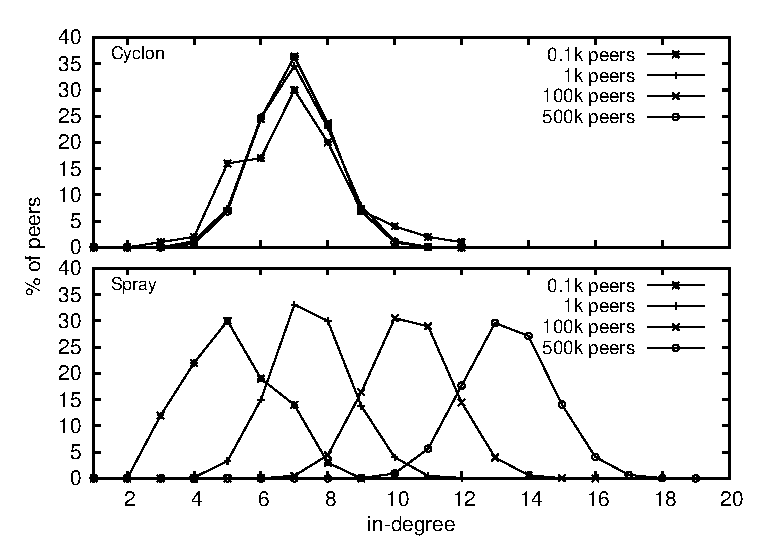
\includegraphics[width=0.49\textwidth]{img/histo.eps}
  \caption{\label{fig:histo}In-degree distribution}
\end{figure}

\begin{asparadesc}
\item[Objective:] As the degree distribution shows the existence of both,
  weakly connected peers as well as strongly connected hubs, it helps to
  analyze the robustness of the overlay when failure is present.  Additionally,
  it indicates how well-distributed links in the network are which
  helps to approximate the resource usage across peers.
\item[Description:] As the overlay can be represented as a directed graph we
  distinguish between out-degree which determines to how many other nodes a
  peer points, and the in-degree which determines from how many other peers a
  certain peer is referenced.  We concentrate on the in-degree for better
  comparison as in \CYCLON{} the out-degree is fixed ($c$).
\item[Results:] Figure~\ref{fig:histo} shows the in-degree distribution of
  \CYCLON{} and \SCAMPLON{}.  In \CYCLON{} the number of peers in the overlay
  has no influence on the degree distribution always as it always gathers
  around the selected partial view size $c$.  In \SCAMPLON{}, however, the
  degree distribution depends logarithmically on the network size and grows and
  shrinks with the network.
\item[Reasons:] \CYCLON{}'s fixed partial view size accounts for its rigid
  behavior.  In \SCAMPLON{} the distribution is much more fluid...
\end{asparadesc}

\subsection{Dynamic network}

\begin{figure}
  \centering
  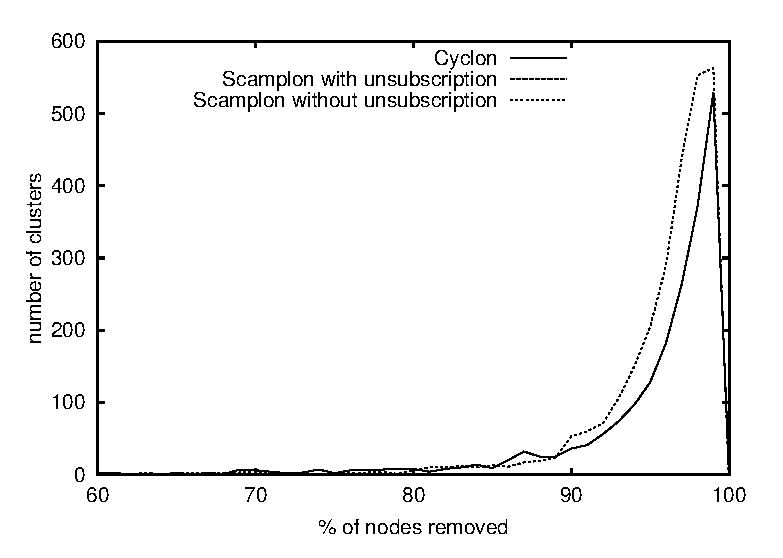
\includegraphics[width=0.49\textwidth]{img/churn.eps}
  \caption{\label{fig:churn}Churn effect}
\end{figure}

\begin{asparadesc}
\item[Objective:] To highlight that \SCAMPLON{} is adaptive, i.e., the total
  number of connections reflects the network membership. Furthermore, the
  connections are quickly spread among the members.
\item[Description:] The first half of the experimentation, $2,500$ peers are
  added $4$ times successively by intervals of $10$ cycles each. Thus, the
  network size goes from $0$ to $10,000$ peers in $40$ rounds. Then, half of
  the network leaves without giving notice ($5,000$ peers). Finally, $2,500$
  peers join two additional times. The final network size is $10,000$
  members. The measurements concern
  \begin{inparaenum}
  \item the number of connections in the network over cycles,
  \item the variance of the partial view sizes over cycles
    (cf. Section~\ref{subsec:cyclic}).
  \end{inparaenum}
\item[Results:] Figure~\ref{fig:churn} shows the result of the experiment. The
  x-axis represents the cycles (i.e. the arbitrary unit time frame). The top
  figure shows the number of connections established in the network (scale
  $\times 10^3$). The bottom figure shows the variance in the partial view size
  of the members. We can see that at each batch of joinings, the connection
  number grows to reflect the needs of the new network membership. The
  observation is consistent with the variance measures. Indeed, at each batch
  of insertions, the variance suddenly grows. Then, it exponentially decreases
  and converges to zero in less than $10$ cycles. The variance is higher when
  the network size is lower. For instance, the first $2,500$ peers lead to the
  highest variance. At the $40^{th}$ rounds, half of the peers
  leave/crash. Around half of the connections are directly removed without
  disturbing the variance of partial views. The $10$ following cycles show a
  slight decrease of connections. Then new members are introduced in the
  network yielding the same results as earlier joinings.
\item[Reasons:] Since the partial views of \SCAMPLON{} adapt themselves to the
  network size, the number of connections grows as the network membership
  grows.  The peaks in variance correspond to the joining parts of the
  experiment. The disparity comes from the fact that new peers arrive in the
  network with a small partial view. The peaks are smaller when the network is
  larger. Indeed, the peers - which already were network members before the new
  arrivals - had a few rounds to exchanges and even up their partial views. As
  consequence, it lessens the weight of joinings. The removal of $5,000$ peers
  do not disturb the variance since they are made at random. Thus, no peers
  suffer more of these removals than others. The slightly decreasing number of
  connections after the removal is due to peers realizing that some connections
  are dead, leading to a probabilistic removal
  (cf. Algorithm~\ref{algo:unreachable}).
\end{asparadesc}

\subsection{Massive failures}
\label{subsec:resilience}

\begin{figure}
  \centering
  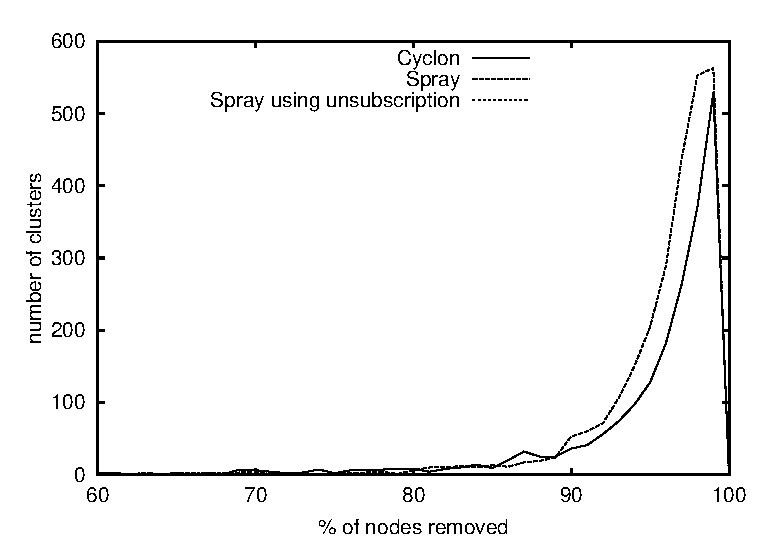
\includegraphics[width=0.49\textwidth]{img/resilience.eps}
  \caption{\label{fig:resilience}Resilience to massive failure}
\end{figure}


\begin{algorithm}

\small
\algrenewcommand{\algorithmiccomment}[1]{\hskip2em$\rhd$ #1}

\newcommand{\comment}[1]{$\rhd$ #1}

\algblockdefx[initially]{initially}{endInitially}
  [0] {\textbf{INITIALLY:}}

\algblockdefx[pas]{pas}{endPas}
  [0] {\textbf{EVENTS:}}

\newcommand{\LINEFOR}[2]{%
  \algorithmicfor\ {#1}\ \algorithmicdo\ {#2} %
  }

\newcommand{\LINEIFTHEN}[2]{%
  \algorithmicif\ {#1}\ \algorithmicthen\ {#2} %
  }

\newcommand{\INDSTATE}[1][1]{\State\hspace{\algorithmicindent}}

\begin{algorithmic}[1]
  \Statex
  \initially
  \State $\mathcal{I}$ \hfill \label{line:inview}
  \comment{set of peers targeting us ($p$) in their partial view}
  \endInitially

  \pas
    \Function{unSubscribe}{\ }
    \For{$i\leftarrow 0$ \textbf{to} $min(|\mathcal{P}|,\, |\mathcal{P}|-1)$ 
      \label{line:bridge}}    
    \State \textbf{let} $\langle n,\,\_ \,\rangle \leftarrow \mathcal{P}[i]$;
    \State $sendTo(\, \mathcal{I}[\,i\%|\mathcal{I}|\,],\, 'unSubs',\, n)$;
    \EndFor
    \EndFunction
    \Statex
    \Function{onUnSubs}{$o, \, n$} 
    \hfill \comment{$o$: origin; $n$: neighbor to add}
    \State $\mathcal{P}\leftarrow (\mathcal{P}\setminus o)
    \uplus\{\langle n,\,0\rangle\}$;
    \EndFunction
  \endPas
\end{algorithmic}

\caption{\label{algo:unsubscription}Unsubscription protocol from
  \SCAMP{}~\cite{ganesh2003peer}}
\end{algorithm}

\begin{asparadesc}
\item[Objective:] 
\item[Description:] Algorithm~\ref{algo:unsubscription} shows the
  unsubscription protocol which guarantees connectedness (WITH HIGH PROBA?)
  upon the assumption that an \emph{in view} $\mathcal{I}$ is maintained
  (cf. Line~\ref{line:inview}) along with bidirectional connections. The set of
  peers which have a particular peer in their partial view populate the
  latter's in view. When a peer leaves, it actively contributes to repair the
  network by acting like a bridge between its in view $\mathcal{I}$ and its
  partial view $\mathcal{P}$. As consequence, the neighbors from $\mathcal{I}$
  add each peer from the leaving peer's partial view in their own partial view.
  Except for one peer (cf. Line~\ref{line:bridge}), it guarantees that these
  peers stay connected, i.e., that at least one partial view references them.

\item[Results:]
\item[Reasons:]
\end{asparadesc}

\subsection{Degeneration}

\begin{figure}
  \centering 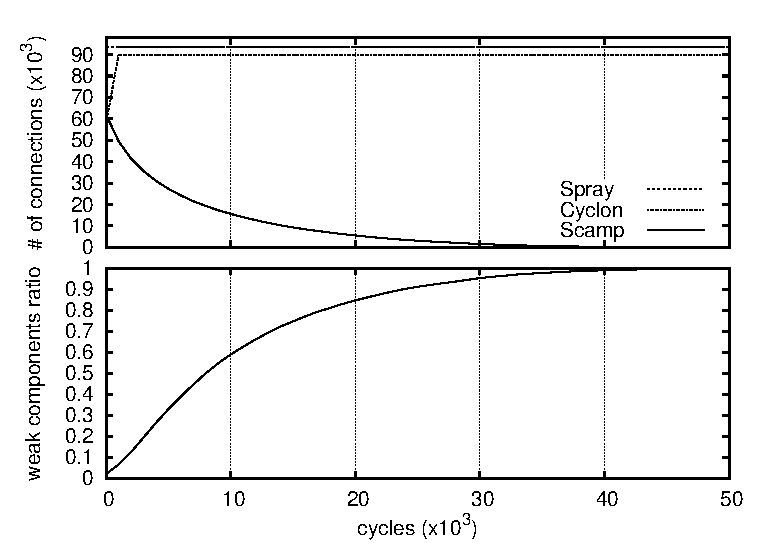
\includegraphics[width=0.49\textwidth]{img/degen.eps}
  \caption{\label{fig:degen}Degeneration of static network} \end{figure}

\begin{asparadesc} \item[Objective:] \SCAMPLON{}, especially when using
        \emph{handshaking}, is vulnerable to message loss. When messages can
        be lost, a static \SCAMPLON{} overlay where peers neither join
        nor leave will slowly degenerate.
        The reason for this can be found in Algorithm~\ref{algo:unreachable} 
        where arcs are potentially lost when a message is lost.
        As static protocols like \CYCLON{} are not prone to this degeneration
        we compare with another adaptive probabilistic protocol,
        \SCAMP{}, instead. We adapted \SCAMP{} so that its lease-mechanism preserves
        the total number of arcs in the network.
        This experiment focuses on two features: the total number of arcs in the 
        graph and the number of weak components.
\item[Description:]
    As previously shown, the number of arcs in the network should be
    $|\mathcal{N}|\log{|\mathcal{N}|}$ for the overlay to be robust. A weak
    component $\mathcal{W}$ of a graph $G$ is a maximum subgraph where the direction
    is ignored.
    Naturally, we want the number of weak components $|\mathcal{W}|$ to be $1$,
    meaning that the whole network is connected.
    When the overlay consists of more than one component, the network is disconnected.
    Unlike with strong component where the direction is taken into account, \SCAMPLON{}
    cannot repair itself when more than one weak component is present.
    The experiment involves handshaking and is conducted with an overlay consisting
    of $10,000$ peers over a period of $100,000$ cycles and a probability of
    $\frac{1}{1000}$ that a link fails. \TODO{BRICE: PLEASE ELABORATE YOUR CALCS}

\item[Results:]
    The x-axis in Figure~\ref{fig:degen} shows the number of cycles the protocol was
    executed.
    The upper graphs y-axis represents the total number of arcs in the
    overlay while the lower graphs y-axis shows the percentage that weak components
    make up of the total network: $\frac{|\mathcal{W}|}{|\mathcal{N}|}$.
    We clearly see that \SCAMPLON{} degenerates much slower than \SCAMP{} and that
    it becomes disconnected very late while \SCAMP{} collapses quickly.

\item[Reasons:]
    As \SCAMP{} must maintain much more links than \SCAMPLON{} when establising a
    connection it has a higher probability of losing arcs which, in turn, let it
    degenerate much quicker.
    Furthermore, while in \SCAMPLON{} we can easily predict if a link failed or if
    the node failed and thus we can stop the degeneration this is not possible in
    \SCAMP{} as it cannot be easiliy predicted for when a link failed due to its
    random walk nature.

\end{asparadesc}

%% \subsection{Synthesis}

%%% Local Variables:
%%% mode: latex
%%% TeX-master: "../paper"
%%% End:
